\documentclass[9pt,a4paper]{extarticle}
\usepackage[top=4mm,bottom=4mm,left=5mm,right=5mm]{geometry}
\usepackage{fontspec}
\usepackage{xeCJK}
\usepackage{xcolor}
\usepackage{graphicx}
\usepackage{tikz}
\usepackage{tabularx}
\usepackage{array}
\usepackage[most]{tcolorbox}
\usepackage[hidelinks]{hyperref}

\pagestyle{empty}
\setmainfont{Times New Roman}
\setCJKmainfont{DFKai-SB}[AutoFakeBold=2]
\urlstyle{same}
\setlength{\parindent}{0pt}
\setlength{\parskip}{0pt}
\renewcommand{\baselinestretch}{0.97}

\definecolor{ink}{HTML}{0B1F3A}
\definecolor{muted}{HTML}{42526B}
\definecolor{soft}{HTML}{F6FAFF}
\definecolor{line}{HTML}{D7E3F3}
\definecolor{blueA}{HTML}{1557C0}
\definecolor{cyanA}{HTML}{008C95}
\definecolor{purpleA}{HTML}{6D35B8}
\definecolor{orangeA}{HTML}{F05A22}
\definecolor{greenA}{HTML}{079669}
\definecolor{redA}{HTML}{C62828}
\definecolor{goldA}{HTML}{D18B00}
\color{ink}

\tcbset{
  resumeBox/.style={
    enhanced,
    boxrule=.72pt,
    arc=2mm,
    left=1mm,
    right=1mm,
    top=.6mm,
    bottom=.6mm,
    colback=white,
    before skip=0pt,
    after skip=0pt,
    fontupper=\color{ink}
  }
}

\newtcolorbox{colorboxx}[2][]{resumeBox,colframe=#2,#1}
\newcommand{\hi}[1]{\textcolor{redA}{\textbf{#1}}}
\newcommand{\muted}[1]{\textcolor{muted}{#1}}
\newcommand{\sect}[3]{%
  \noindent{\large\bfseries\textcolor{#2}{#1}}\hspace{1mm}{\large\bfseries #3}\par\vspace{0.35mm}
}
\newcommand{\chip}[2]{%
  \tcbox[
    enhanced,
    on line,
    boxrule=.45pt,
    arc=1.4mm,
    left=.75mm,
    right=.75mm,
    top=.35mm,
    bottom=.35mm,
    colback=#1!7,
    colframe=#1!70,
    boxsep=0pt
  ]{\scriptsize\bfseries\textcolor{#1}{#2}}%
}
\newcommand{\point}[2]{%
  {\scriptsize\textcolor{#1}{\bfseries #2}}\par
}
\newcommand{\tinyline}[2]{%
  {\footnotesize\textbf{#1}}\ {\footnotesize #2}\par
}
\newcommand{\proofimg}[3]{%
  \begin{minipage}[t]{#1}
    \centering
    \fcolorbox{line}{white}{\includegraphics[width=\dimexpr\linewidth-2\fboxsep-2\fboxrule,height=16mm,keepaspectratio]{#2}}\\[-.3mm]
    {\scriptsize\bfseries #3}
  \end{minipage}
}

\begin{document}
\begin{tikzpicture}[remember picture,overlay]
  \fill[soft] (current page.south west) rectangle (current page.north east);
  \foreach \x in {0,9,...,210} \draw[line,opacity=.34,line width=.16pt] ([xshift=\x mm]current page.south west) -- ([xshift=\x mm]current page.north west);
  \foreach \y in {0,9,...,297} \draw[line,opacity=.34,line width=.16pt] ([yshift=\y mm]current page.south west) -- ([yshift=\y mm]current page.south east);
  \fill[blueA!12] ([xshift=136mm,yshift=271mm]current page.south west) .. controls +(18mm,18mm) and +(-10mm,18mm) .. ([xshift=206mm,yshift=265mm]current page.south west) -- ([xshift=206mm,yshift=297mm]current page.south west) -- ([xshift=146mm,yshift=297mm]current page.south west) -- cycle;
  \draw[blueA,opacity=.16,line width=1.2pt] ([xshift=7mm,yshift=244mm]current page.south west) -- ([xshift=205mm,yshift=284mm]current page.south west);
  \draw[purpleA,opacity=.18,line width=1pt] ([xshift=164mm,yshift=294mm]current page.south west) -- ([xshift=210mm,yshift=252mm]current page.south west);
\end{tikzpicture}

\begin{minipage}[t]{36mm}
  \begin{colorboxx}[height=39mm,valign=center,halign=center]{blueA}
    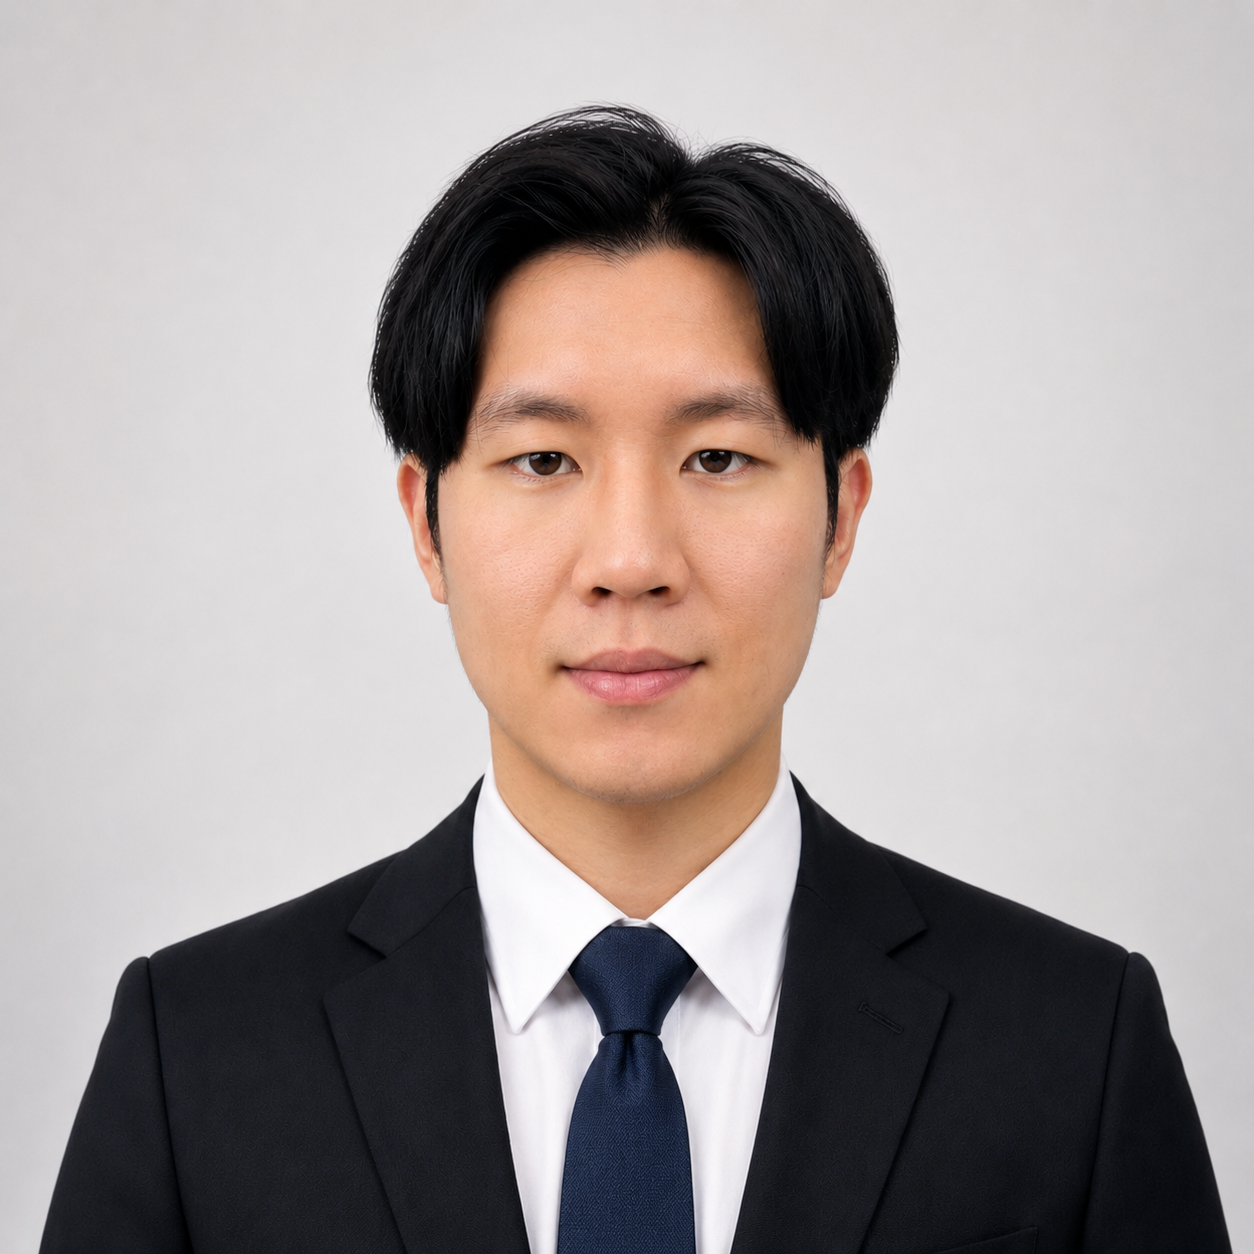
\includegraphics[width=30mm,height=35mm,keepaspectratio]{assets/profile-photo.png}
  \end{colorboxx}
\end{minipage}\hfill
\begin{minipage}[t]{103mm}
  {\fontsize{25}{26}\selectfont\bfseries\textcolor{ink}{呂哲言}}\par\vspace{.3mm}
  {\fontsize{14}{16}\selectfont\bfseries\textcolor{blueA}{AI / LLM / RAG / Multimodal AI Engineer}}\par
  {\small 淡江大學資訊工程學系 \textbf{學士畢業｜碩士畢業}}\par\vspace{1.4mm}
  \tinyline{Email：}{a28473458@gmail.com}
  \tinyline{LINE ID：}{david891205}
  \tinyline{作品集：}{\href{https://david891205.github.io/resume-site/}{david891205.github.io/resume-site}}
  \vspace{1mm}
  {\footnotesize\bfseries
    \textcolor{blueA}{專長大型語言模型、RAG、AI Agent、多模態 AI 與 NLP 系統開發}\par
    \textcolor{ink}{具 \hi{產學合作}、\hi{競賽獲獎}、\hi{企業導入} 與工作坊教學經驗}
  }
\end{minipage}\hfill
\begin{minipage}[t]{45mm}
  \begin{colorboxx}[height=39mm,valign=center]{purpleA}
    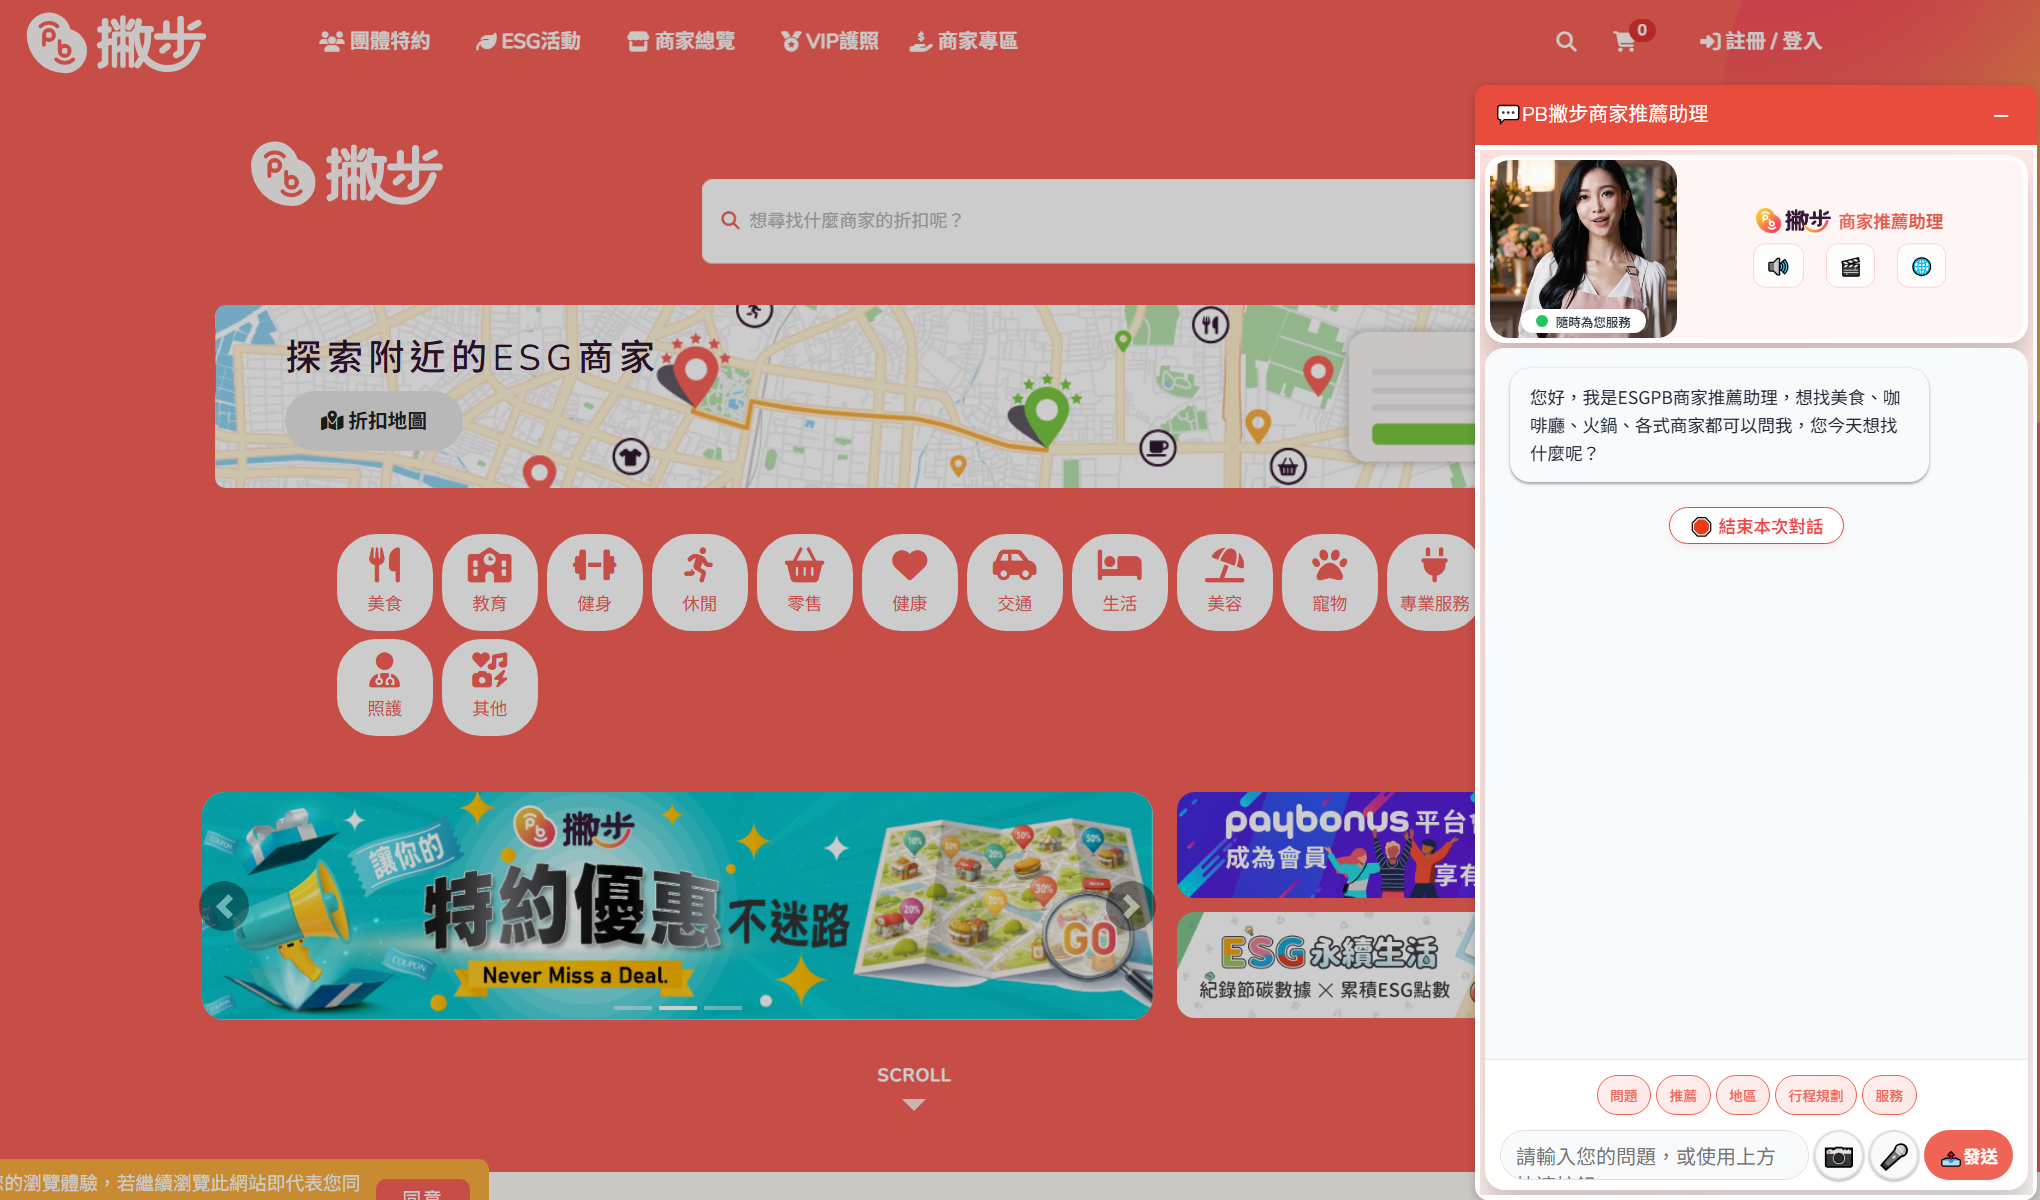
\includegraphics[width=\linewidth,height=18mm,keepaspectratio]{assets/esgpb-chatbot-screenshot.png}\par\vspace{.45mm}
    {\footnotesize\bfseries\textcolor{purpleA}{可展示系統}}\par
    {\footnotesize ESGPB 商家推薦助理、智慧旅遊、會議秘書、醫療工作坊與鐵道 AI 技術服務。}
  \end{colorboxx}
\end{minipage}

\vspace{.9mm}
\begin{tabularx}{\linewidth}{@{}XXXX@{}}
\begin{colorboxx}[height=13mm,valign=center]{blueA}
  {\large\bfseries\textcolor{blueA}{2025}}\par
  {\footnotesize 台灣服務創新獎｜\hi{代表領獎}}
\end{colorboxx}
&
\begin{colorboxx}[height=13mm,valign=center]{cyanA}
  {\large\bfseries\textcolor{cyanA}{InnoServe}}\par
  {\footnotesize 商業發展治理創新組｜\hi{第三名}}
\end{colorboxx}
&
\begin{colorboxx}[height=13mm,valign=center]{purpleA}
  {\large\bfseries\textcolor{purpleA}{AI 應用鬥智賽}}\par
  {\footnotesize Deep龍力｜\hi{佳作}}
\end{colorboxx}
&
\begin{colorboxx}[height=13mm,valign=center]{orangeA}
  {\large\bfseries\textcolor{orangeA}{5+}}\par
  {\footnotesize 產學 / 研究 / 教學 AI 專案}
\end{colorboxx}
\end{tabularx}

\vspace{.9mm}
\begin{minipage}[t]{99mm}
  \begin{colorboxx}[height=38mm]{blueA}
    \sect{1}{blueA}{核心技能}
    \chip{blueA}{Python}\hspace{.6mm}
    \chip{blueA}{PyTorch}\hspace{.6mm}
    \chip{blueA}{Transformers}\hspace{.6mm}
    \chip{blueA}{Hugging Face}\hspace{.6mm}
    \chip{cyanA}{RAG}\hspace{.6mm}
    \chip{cyanA}{LangChain}\hspace{.6mm}
    \chip{cyanA}{LangGraph}\hspace{.6mm}
    \chip{cyanA}{OpenAI API}\hspace{.6mm}
    \chip{orangeA}{FastAPI}\hspace{.6mm}
    \chip{orangeA}{Docker}\hspace{.6mm}
    \chip{orangeA}{Qdrant}\hspace{.6mm}
    \chip{orangeA}{Redis}\hspace{.6mm}
    \chip{orangeA}{PostgreSQL}\hspace{.6mm}
    \chip{purpleA}{Whisper}\hspace{.6mm}
    \chip{purpleA}{OpenCV}\hspace{.6mm}
    \chip{purpleA}{Blip2}\hspace{.6mm}
    \chip{purpleA}{Pose Estimation}\hspace{.6mm}
    \chip{purpleA}{3DCNN}\hspace{.6mm}
    \chip{greenA}{Multimodal Fusion}\hspace{.6mm}
    \chip{greenA}{Error Analysis}
    \vspace{.6mm}

    {\footnotesize
    \textbf{能交付：}資料清理、向量檢索、對話記憶、語音 / 圖片輸入、後端 API、展示流程與技術文件。}
  \end{colorboxx}
\end{minipage}\hfill
\begin{minipage}[t]{94mm}
  \begin{colorboxx}[height=38mm]{cyanA}
    \sect{2}{cyanA}{學歷與研究}
    {\small\bfseries 淡江大學｜資訊工程學系 學士畢業、碩士畢業}\par\vspace{.45mm}
    {\footnotesize
    \textbf{碩士論文方向：}開放域目標導向主動對話，研究模型如何依對話歷史、候選知識與目標推進回應。}\par\vspace{.65mm}
    {\footnotesize
    \textbf{研究重點：}BART、GPT-2、DPO、對比學習、Dialogue Planning、Response Generation。}\par\vspace{.65mm}
    {\footnotesize
    \textbf{實作重點：}資料處理、模型訓練、評估指標、錯誤分析與可重現實驗。}
  \end{colorboxx}
\end{minipage}

\vspace{.9mm}
\begin{colorboxx}{purpleA}
  \sect{3}{purpleA}{代表專案}
  \begin{tabularx}{\linewidth}{@{}X X@{}}
  \begin{colorboxx}[height=20mm]{blueA}
    {\small\bfseries 全域意境感知智慧會議秘書系統}\par
    {\footnotesize AIGO 佳作相關技術文件｜Whisper、說話者分離、Sentence-BERT、TextRank、LLM、n8n / Webhook。}\par
    {\footnotesize 我負責把會前資料、會中摘要、會後任務追蹤串成可展示流程。}
  \end{colorboxx}
  &
  \begin{colorboxx}[height=20mm]{cyanA}
    {\small\bfseries ESGPB 虛擬人商家推薦助理}\par
    {\footnotesize 好奇兄弟雲端合作｜RAG、Qdrant、Redis、PostgreSQL、GPT Realtime、Sora。}\par
    {\footnotesize 串接商家資料 API，支援優惠推薦、語音、文字與拍照互動。}
  \end{colorboxx}
  \end{tabularx}
  \vspace{.8mm}
  \begin{tabularx}{\linewidth}{@{}X X@{}}
  \begin{colorboxx}[height=20mm]{purpleA}
    {\small\bfseries InnoServe 第三名｜多模態旅遊 AI Agent}\par
    {\footnotesize 具意圖探測的多模態旅遊問答服務系統｜Neo4j、Qdrant、Whisper、Blip2、LLM。}\par
    {\footnotesize 支援行程問答、導遊減勞與旅後分析，獲商業發展治理創新組第三名。}
  \end{colorboxx}
  &
  \begin{colorboxx}[height=20mm]{orangeA}
    {\small\bfseries 112 霸凌偵測及專注力辨識系統}\par
    {\footnotesize 精英國際教育集團｜科技部案｜STT、BERT、MFCC、CNN/LSTM、3DCNN、多模態融合。}\par
    {\footnotesize 協助疑似霸凌與專注力狀態偵測，讓幼教場域能即時介入。}
  \end{colorboxx}
  \end{tabularx}
\end{colorboxx}

\vspace{.9mm}
\begin{minipage}[t]{99mm}
  \begin{colorboxx}[height=45mm]{orangeA}
    \sect{4}{orangeA}{獲獎與成果}
    {\footnotesize
    \textbf{2025 InnoServe｜商業發展治理創新組 \hi{第三名}}\par
    作品：具意圖探測的多模態旅遊問答服務系統。\par\vspace{.8mm}
    \textbf{2024 年度 AI 應用鬥智賽｜Deep龍力 \hi{佳作}}\par
    議題：以 Llama 為例解決 LLM 幻覺問題、節省成本及特殊需求。\par\vspace{.8mm}
    \textbf{2025 第十屆台灣服務創新獎｜\hi{代表領獎}}\par
    代表 AIIT 淡江大學人工智慧與產業技術實驗室領取 AI 應用相關成果。\par\vspace{.55mm}
    \textbf{國科會 / 科技部案與產學合作 AI 專案 5+}\par
    教育安全、英語學習、智慧照護、高齡健康、ESG 商家推薦、鐵道巡檢與醫療工作坊。\par\vspace{.55mm}
    \textbf{面試可直接看：}獎狀、公開頁、ESGPB 截圖、PPT 預覽、展示影片、活動照片與合作連結。}
  \end{colorboxx}
\end{minipage}\hfill
\begin{minipage}[t]{94mm}
  \begin{colorboxx}[height=45mm]{greenA}
    \sect{5}{greenA}{研究 / 計畫 / 教學}
    {\footnotesize
    \textbf{國科會 / 科技部案：}\par
    112年度「產學合作計畫-基於深度學習之霸凌偵測及專注力辨識系統」【科技部案】。\par
    113年度「產學合作計畫—AI智慧英語學習系統之開發及融入精準學習之成效」【科技部案】。\par
    智慧居家養老~基於機器學習與深度學習的規律性分析、行為辨識及異常狀態辨識研究與實作。\par
    高齡者智慧健康管理：基於 AI 姿勢分析與知識圖譜問答【科技部案】。\par\vspace{.45mm}
    \textbf{工作坊與課程：}榮總 AI 輔助預立醫療流程工作坊、陽明交通大學半導體 AI 與 ChatGPT 應用班。\par\vspace{.45mm}
    \textbf{可追問能力：}多模態資料融合、RAG 架構、語音互動、API 串接、醫療 / 教育 / 工程場域文件整理。}
  \end{colorboxx}
\end{minipage}

\vspace{.9mm}
\begin{colorboxx}{blueA}
  \sect{6}{blueA}{企業合作與證據}
  \begin{minipage}[t]{78mm}
    {\footnotesize
    \textbf{台灣世曦工程：}協助「委託應用AI建構鐵道專業服務及巡檢數位轉型建置之規劃、基本設計、細部設計審查、監督審驗(含鐵道領域專業顧問)技術服務」內容整理。\par
    \textbf{可查資料：}作品集內有獎狀、ESGPB 截圖、簡報預覽、會議諸葛影片、榮總工作坊照片、世曦工程合照與公開連結。\par\vspace{.8mm}
    \textbf{完整作品集：}代表專案包含需求、我的角色、技術流程、Demo / 獎項 / 照片證據。}
  \end{minipage}\hfill
  \begin{minipage}[t]{111mm}
    \proofimg{34mm}{assets/innoserve-travel-award.jpg}{InnoServe}\hfill
    \proofimg{34mm}{assets/aigo-deeplong-award.jpg}{Deep龍力}\hfill
    \proofimg{34mm}{assets/service-award-stage.jpg}{服務創新獎}\par\vspace{.7mm}
    \proofimg{34mm}{assets/esgpb-chatbot-screenshot.png}{ESGPB}\hfill
    \proofimg{34mm}{assets/vgh-ai-workshop-speaking.jpg}{榮總工作坊}\hfill
    \proofimg{34mm}{assets/ceci-ai-railway-visit.png}{世曦工程}
  \end{minipage}
\end{colorboxx}

\vspace{1.1mm}
\begin{tcolorbox}[
  enhanced,
  boxrule=0pt,
  arc=0mm,
  left=2mm,
  right=2mm,
  top=1mm,
  bottom=1mm,
  colback=blueA,
  coltext=white
]
  {\large\bfseries 研究 × 實作 × 產學合作 × 企業導入}\hfill
  {\small 用 AI 驅動價值，以能被展示與追問的成果說話}
\end{tcolorbox}

\end{document}
